\section{Dual conics}

\subsection*{Definition}
\begin{definition}
    A \emph{dual conic} is a set of lines $l$ that satisfy equation:
    \[l^TC^{*}l=0\]
    where $C^{*}$ is a $3 \times 3$ symmetric matrix.

    A \emph{non-degenerate dual conic} is a dual conic whose matrix $C^{*}$ is non-singular: 
    \[\textnormal{rank}(C^{*})=3\]
\end{definition}
Consider a non-degenerate conic, denoted as $C$, and the collection of all lines $l$ that are tangents to it.
For each point $c$ on the conic $C$, there exists a line $l$ that is tangent to $C$. 
Since $l$ is the polar line of $x$ with respect to $C$, we can express it as $l=Cc$.
Consequently, we can represent $x$ as:
\[x=C^{-1}l\]
Moreover, given that $C$ is a symmetric matrix, we have:
\[x^T=l^Tl^{-T}=l^TC^{-1}\]
Now, considering that the point $x$ lies on the conic $C$, we have:
\[x^TCx=0\]
By substituting the previously derived expressions, we arrive at:
\[l^TC^{-1}l=0\]
This equation represents a quadratic homogeneous equation on $l$. 
Therefore, we can conclude that for the dual conic holds $C^{*}=C^{-1}$. 
We can also note that a non-degenerate dual conic $C^{*}$ is the collection of lines that are tangent to a non-degenerate conic $C$.

\subsection*{Degenerate dual conics}
\begin{definition}
    A \emph{degenerate dual conic} is a conic where the matrix $C^{*}$ is singular: 
    \[\textnormal{rank}(C^{*}) < 3\]
\end{definition}
There are two possible scenarios to consider:
\begin{itemize}
    \item When $\textnormal{rank}(C^{*}) = 2$, any symmetric $3 \times 3$ matrix $C^{*}$ can be expressed as:
        \[C^{*}=pq^T+qp^T\]
        In this case, the conic represents the line $l$ passing through point $p$ or the line $l$ passing through point $q$.
        \begin{figure}[H]
            \centering
            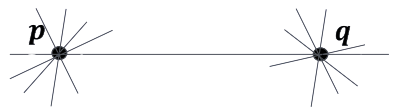
\includegraphics[width=0.25\linewidth]{images/deg2.png}
        \end{figure}
    \item When $\textnormal{rank}(C^{*}) = 1$, any symmetric $3 \times 3$ matrix $C^{*}$ can be expressed as:
        \[C^{*}=pp^T\]
        In this situation, the conic corresponds to the line $l$ going through point $p$ repeated twice. 
        \begin{figure}[H]
            \centering
            
\includegraphics[width=0.1\linewidth]{images/deg1.png}
        \end{figure}
\end{itemize}

\begin{definition}
    The degenerate dual conic $C^{*}=pq^T+qp^T$ going through two circular point $p$ and $q$ is known as the \emph{conic dual to the circular points}, and it can be expressed as:
    \[C^{*}_{\infty}=IJ^{T}+JI^{T}=
    \begin{bmatrix}
        1 & 0 & 0 \\
        0 & 1 & 0 \\
        0 & 0 & 0 
    \end{bmatrix}\]
\end{definition}